 % This example An LaTeX document showing how to use the l3proj class to
% write your report. Use pdflatex and bibtex to process the file, creating 
% a PDF file as output (there is no need to use dvips when using pdflatex).

% Modified 

\documentclass{l3proj}
\begin{document}
\title{Team V - How Not To Kill Your Dog}
\author{Ross Adam \\
        Andrew Gardner \\
        Nicole Kearns \\
        Mamas Nicolaou \\
        Asset Sarsengaliyev}
\date{18 March 2013}
\maketitle
\tableofcontents

\chapter{Evaluation and Testing}
\label{evaluation}

This section discusses the methods used for testing and evalutating our application. Testing is important in order to ensure that all requirements are met and to identify and rectify any errors. Using various methods of evaluating allows us to test the usability and functionality of our final application.

\section{Testing}

\subsection{Test Plan and Strategy}

Firstly, we created a test log in which we added the feature tested, the date it was tested and the result of the test. Each time we tested a new feature it was added to the test log in order to keep track of what had been tested and whether or not it had been successful.

Initially, for testing our application, we tested each new feature as they were implemented. After running the application to see if the new feature worked as expected, we then tested it with the previous feature already implemented to ensure that they didn't conflict or cause the application to crash.

If an error was detected or the feature caused the application to crash, this was documented in the test log and was raised as an issue on the team's GitHub. It was then assigned to a developer so that the issue could be diagnosed and fixed. Doing this allowed us to keep track of any and all issues and errors that had occurred throughout the implementation process.

However, we found that this was very time consuming, as opposed to having a pre-defined set of test scripts. We then created a set of test scripts for each page within the application. After implementing a several features, we would run the test-script in order to see if they worked as expected and produced the correct output.\\
This will give us a generic view of our applications status. This would dynamically generate a pie chart to give a visual presentation of the number of 'Passed', 'Failed' and 'Blocked' tasks.

\begin{itemize}
\item Passed Result - a test task that runs successfully and produces the expected result.
\item Failed Result - a test task that does not produce the expected result.
\item Blocked Result - A test task that cannot be run, due to an issue thats waiting to be resolved. For example, if the answer validation function is not yet implemented, then a test that includes answer validation cannot be run.
\end{itemize}

\subsection{Issues}

Some of the main issues we encounter are listed below.

\begin{center}
Table 6.1 - Main issues occurred throughout development\\
\begin{tabular}{|c|c|}
\hline \textbf{Issue} & \textbf{Current Status}\\
\hline 
\hline ImageField throws 404 error when trying to access saved Image & Resolved\\
\hline No error for 0 slides in a topic & Resolved\\
\hline Application crashes when clicking next topic button & Resolved\\
\hline Application font appears different on different web-browsers & Unresolved\\
\hline System returns "Wrong answer" for correct answer. & Resolved\\
\hline Questions in final assessment are not displayed in random order & Resolved\\
\hline
\end{tabular}\\
\textit{{\small The table shows some issues which we encountered throughout the development of our application.}}
\end{center}


% Bugs 
% ImageField throws 404 error when trying to access saved Image
% No error for 0 slides in a topic
% Topic id not updating - had to use a topic list.

\subsection{Testing Results Sample}

An example test script can be seen in Figure ..... This includes a set of tasks with their expected behaviour and the results achieved in each test cycle. 

\begin{figure}[!htb]
\caption{Test Script Example}
 \centering
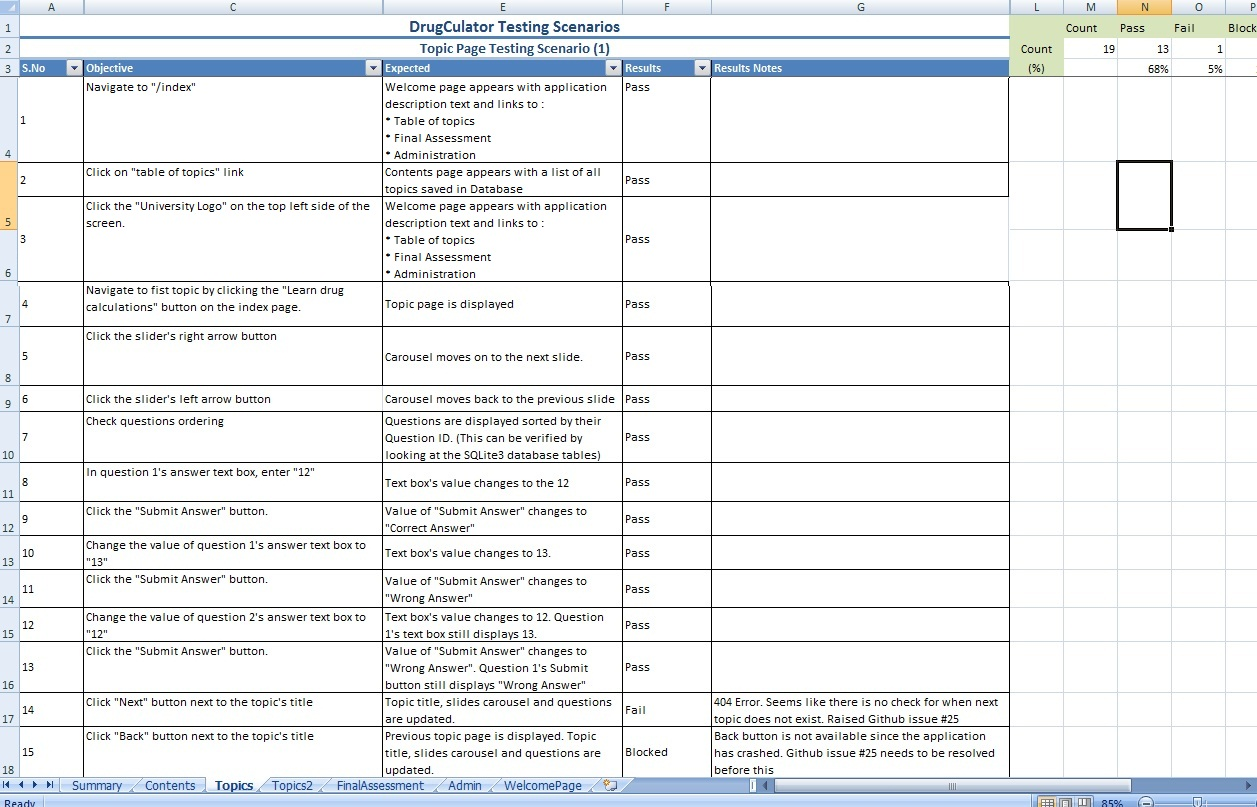
\includegraphics[width=0.7\textwidth]{/users/level3/1002336a/TP3/team-project/Dissertation/images/TopicTest.jpg}
\end{figure}


Figure ..... below shows the test results summary for all the test scripts produced. 

\begin{figure}[!htb]
\caption{Test Results Summary Example}
 \centering
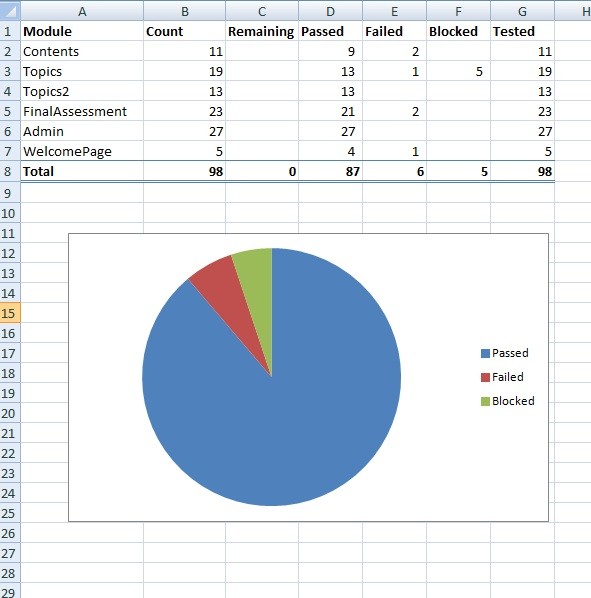
\includegraphics[width=0.5\textwidth]{/users/level3/1002336a/TP3/team-project/Dissertation/images/TestResultsSummary.jpg}
\end{figure}

\section{User Evaluation}

In order to test the usability and functionality of our application, we identified the features of the application which would provide us with the most accurate results:

\begin{itemize}
\item Content management; admin users should be able to easily upload, edit and delete content.
\item Browse through topics successfully.
\item Answer all questions available.
\item Complete the final assessment and see their final score. 
\end{itemize}

We then created a test plan to evaluate the usability and likeability of the application. To test both the administration features and the learning functionality for the students, we created a set of tasks based on the features above. We used the 'Think-Aloud' method during the evaluation and provided participants with a short questionnaire afterwards.

\subsection{Functional Requirement Fulfilment}

%At this point in time all of the client's requirements have been met. This application's implementation has been very iterative.
%Meeting with our client repeatedly over the course of development has meant that we have been steadily improving the application and refactoring our code. 
%
%Developing beyond the must have requirements we have developed a game-ified final assessment page and also refined our application design to increase usability and aesthetic appeal for the end user.

Before carrying out our evaluation with a group of participants, our team carried out an evaluation on ourselves in order to test the application for issues and to see how many of the requirements were satisfied. From this evaluation, we found that our application satisfies each of the clients 15 specified functional requirements. The admin user is able to upload new content, edit content and delete content. The student user can view all topics available and see all related slides and questions for each topic. The student user can also complete the final assessment and see their final score, indicating how well they answered.

The applications implementation has been a very iterative process, and meeting with our client repeatedly over the course of the development has meant that we have been steadily improving the application and refactoring our code.

Developing beyond the 'must have' requirements, we have developed a game-like final assessment page and also refined our application design to increase usability and aesthetic appeal for the end user.


\subsection{Users}

Firstly, we wanted to do an evaluation with our client, Dr Fiona Dowell. This would allow us to see how satisfied our client was with the application we had created and allow us to receive any feedback. Following that, we wanted to get a mixture of Computing Science/Software Engineering students and other students to evaluate our application. As the Computing Science/Software Engineering students had done coursework with Django recently, we thought that having participants who are unfamiliar with Django would provide us with more reliable results for our evaluation.

\subsection{Tasks}

We asked the participants to carry out a number of tasks in order to evaluate our application. We have tasks for both an admin user, to test the administration features and content management, and for a student user, to test the functionality and usability of the learning features.
\newpage

\textbf{Admin User Tasks}

\begin{center}
Table 6.2 - Admin User Tasks
\begin{tabular}{|c|c|}
\hline & \textbf{Task}\\
\hline
\hline 1 & Login as administrator.\\
\hline 2 & Add a new user.\\
\hline 3 & Set the users permissions to allow them to update content - topics, slides, questions.\\
\hline 4 & Add a new Topic.\\
\hline 5 & Add a new slide to that topic.\\
\hline 6 & Go to Topic 2 and remove slide 3.\\
\hline 7 & Add a new question to Topic 1.\\
\hline 8 & Edit question 2 within Topic 2.\\
\hline
\end{tabular}\\
\textit{{\small This table shows the tasks to be carried out by partipants in order to evaluate the admin user functionality.}}
\end{center}

\textbf{Student User Tasks}

\begin{center}
Table 6.3 - Student User Tasks\\
\begin{tabular}{|c|c|}
\hline & \textbf{Task}\\
\hline
\hline 1 &  Go to Topic 1 and browse through the slides.\\
\hline 2 & Answer 2 questions within Topic 1.\\
\hline 3 & Go to Topic 2.\\
\hline 4 & Go to the final Assessment and complete the test.\\
\hline
\end{tabular}\\
\textit{{\small This table shows the tasks to be carried out by participants in order to evaluate the student user functionality.}}
\end{center}

\textbf{User Consent}

In order to avoid any ethical issues, all participants were issued a consent form, which informed them what the testing would involve and what exactly it was for.  It also stated that the participant information would be kept private and that they are able to leave the testing at any time if they did not wish to continue. The consent forms had to be signed and returned before any testing was allowed to commence.

\textbf{Think-Aloud}

All evaluations were performed using the Think Aloud method which involves observing the participants performing the tasks and having them describe out loud what they are doing and why. This is a useful evaluation method as it allows us to see first-hand the process that the participants go through to complete the tasks and highlights any difficulties or errors they may encounter.

\textbf{Questionnaire}

After the evaluation, each participant was asked to complete a quick questionnaire about the application and the tasks they had completed, and provide any additional feedback. The first 4 questions are related to the usability of the content admin tasks, and questions 5 to 8 are about the usability of the student user tasks.

\begin{center}
Table 6.4 - Questionnaire\\
\begin{tabular}{|p{2cm}|p{12cm}|}
\hline & \textbf{Questions} \newline \newline Key: 1 - very easy; 5 - very difficult \\
\hline
\hline 1 & Overall, how easy was the admin system to use? \newline 1 ~~~~~~~~~~ 2 ~~~~~~~~~~ 3 ~~~~~~~~~~ 4  ~~~~~~~~~~ 5\\
\hline 2 & How difficult did you find it to add a new user to the system?  \newline 1 ~~~~~~~~~~ 2 ~~~~~~~~~~ 3 ~~~~~~~~~~ 4  ~~~~~~~~~~ 5\\
\hline 3 & Were you able to change a users access permissions? If so, how difficult was this?  \newline 1 ~~~~~~~~~~ 2 ~~~~~~~~~~ 3 ~~~~~~~~~~ 4  ~~~~~~~~~~ 5\\
\hline 4 & How easy was it to add new content - topics, slides, questions?  \newline 1 ~~~~~~~~~~ 2 ~~~~~~~~~~ 3 ~~~~~~~~~~ 4  ~~~~~~~~~~ 5\\
\hline 5 & Overall, how easy was the application interface to use?  \newline 1 ~~~~~~~~~~ 2 ~~~~~~~~~~ 3 ~~~~~~~~~~ 4  ~~~~~~~~~~ 5\\
\hline 6 & How easy was it to navigate to different topics?  \newline 1 ~~~~~~~~~~ 2 ~~~~~~~~~~ 3 ~~~~~~~~~~ 4  ~~~~~~~~~~ 5\\
\hline 7 & Were you able to browse through slides and questions? If so, how difficult was this?  \newline 1 ~~~~~~~~~~ 2 ~~~~~~~~~~ 3 ~~~~~~~~~~ 4  ~~~~~~~~~~ 5\\
\hline 8 & Were you able to see your final score on the Final Assessment? If so, how clear was this?  \newline 1 ~~~~~~~~~~ 2 ~~~~~~~~~~ 3 ~~~~~~~~~~ 4  ~~~~~~~~~~ 5\\
\hline & Additional Comments \newline\newline \\
\hline
\end{tabular}
\textit{{\small The table above shows the questionnaire each participant completed in order to evaluate the difficulty of the tasks, on a scale of 1 to 5.}}
\end{center}

\subsection{Results}

Overall, the data collected from all the evaluations was positive. However a few suggestions were made for ways to make some tasks more user-friendly and easier to use.\\
While each participant was completing the set of tasks, the time it took for each was recorded. This is important as the amount of time taken can indicate how easy or difficult that task was to complete. 
\newpage
\textbf{Admin User Task Results}

The table below shows the average times for the admin user tasks.

\begin{center}
Table 6.5 - Admin User Results\\
\begin{tabular}{|c|c|}
\hline \textbf{Task Number} & \textbf{Average Time Taken (seconds)}\\
\hline
\hline 1 & 20\\
\hline 2 & 24\\
\hline 3 & 55\\
\hline 4 & 44\\
\hline 5 & 23\\
\hline 6 & 33\\
\hline 7 & 21\\
\hline 8 & 22\\
\hline & n=11\\
\hline
\end{tabular}\\
\textit{{\small This table shows the average times the 11 participants took for each of the admin user tasks.}}
\end{center}

From Table 6.5, it its clear that most participants found task 3, setting the user permissions, the longest task to do. Most users were unsure what access different users were supposed to have and found that there were too many options which made it difficult to find the correct permissions to set.\\
Due to the users and topics being within different sections in the administration page, most participants were unable to locate the 'Topics' section once they had completed the new users tasks, resulting in task 4 taking them longer to complete.\\
Task 6, deleting a slide,  also proved to be slightly time consuming for some users. To delete an item from a topic, the user has to tick the delete check-box for that item and select 'Save'. However, some participants were expecting immediate, visual feedback, once they had selected the delete check-box , to indicate that the item had been deleted and were unaware that to remove it from the topic they had to click the 'Save' button at the bottom of the page.\\

\textbf{Student User Task Results}

The table below shows the average time taken for each of the tasks carried out for the student user.

\begin{center}
Table 6.6 - Student User Results\\
\begin{tabular}{|c|c|}
\hline \textbf{Task Number} & \textbf{Average Time Taken (seconds)}\\
\hline
\hline 1 & 17\\
\hline 2 & 20\\
\hline 3 & 7\\
\hline 4 & 62\\
\hline & n=11\\
\hline
\end{tabular}\\
\textit{{\small This table shows the average times the 11 participants took for each of the student user tasks.}}
\end{center}


As shown in Table 6.6, it is clear that participants had very little problems carrying out the tasks for the student user. The time taken task 4 is quite large due to having to answer all the questions within the Final Assessment. The only problem the participants faced was that most were unaware that the submit button had to be selected for each question, so after answering all the questions, they had to go back to the top of the assessment and select the 'Submit' button for each question.

\textbf{Questionnaire Results}

After completing both sets of tasks, each participant was asked to complete a short questionnaire, containing questions about the usability of the application. The table below shows the average difficulty results from the questionnaires.

\begin{center}
Table 6.7 - Questionnaire Results\\
\begin{tabular}{|c|c|}
\hline \textbf{Question Number} & \textbf{Average Result}\\
\hline
\hline 1 & 2.18\\
\hline 2  & 1.45\\
\hline 3 & 2.36\\
\hline 4 & 1.54\\
\hline 5 & 1.45\\
\hline 6 & 1.09\\
\hline 7 & 1.00\\
\hline 8 & 1.09\\
\hline & n=11\\
\hline
\end{tabular}\\
\textit{{\small The table above shows the average difficulty result from the 11 participants involved, with 1 being very easy and 5 being very difficult.}}
\end{center}

Table 6.7 shows that, overall, the participants found the application easy to use, particuarly the student user tasks.
Although the average results does not indicate that participants had any real difficulty with setting the permissions of users, it is clear from the questionnaire that the participants found this the most difficult task to complete.

\subsection{Feedback}

After completing the questionnaire, participants were asked if they had any additional comments or feedback about the application. Overall, the participants were pleased with the application and found it very simple to use. Some improvements were suggested for both the student view of the application and the administration page.

For the application, although the participants enjoyed the gamification of the Final Assessment with the health bar of the animal, it was suggested by a number of the participants to have a 'Submit All' button to avoid having to submit all answers individually.\\
Another suggestion was to have the sample questions within each topic provide some sort of visual feedback to indicate more clearly to the users if they have the answered the question correctly, for example, change the 'Submit' button to green if correct or red if incorrect.\\
Within the topics, there are 'Next' and 'Previous' links in order to change quickly between the topics without having to repeatedly go to the Table of topics page to select the next topic. However, most particpants did not notice these links, so it was suggested that the size of the text is increased or changed to buttons to make them stand-out and more obvious to the user.

For the admisitration of the application and the users, some participants found that when deleting items from the application, it wasn't obvious how to do this and once they figured it out, they were unsure if the item had actually been deleted. So, it was suggested that there is a delete button for each item, instead of a checkbox, and when clicked the user to receive some immediate, visual feedback to show that the item has been deleted.\\ 
Most of the participants had some difficulty when it came to setting the user permissions as they found that it was not clear what permissions each type of user was supposed to have. Some of the participants suggested that users are added to  'User Groups' which have different levels of access and permissions, and when adding a new user, you can simply select the user group to add them to, avoiding having to set permission individually for each user account created for the application.

\end{document}
